\chapter{Evaluation}
\label{chapter:evaluation}

% \definecolor{win}{HTML}{0de929}
% \definecolor{loss}{HTML}{ef4748}

\definecolor{win}{HTML}{63be7b}
\definecolor{loss}{HTML}{f8696b}

TODO:

definition der testszenarien (was vergleichen wir, warum, wie)

hier ersteinmal leichte Vergleiche (z.B. greedy, random)

\begin{figure}[!ht]
    \centering
    \resizebox{\textwidth}{!}{\begin{tikzpicture}
            \coordinate (bar1Start) at (0,0);
            \coordinate (bar1End) at (10,0);
            \coordinate (bar1Break) at (2.1,0);

            \draw[color=win, line width=0.25cm] (bar1Start) -- (bar1Break);
            \draw[color=loss, line width=0.25cm] (bar1Break) -- (bar1End);
            \node[left = 0.1cm of bar1Start] {Random Player};
            \node[right = 0.1cm of bar1End, align=left] {Greedy Player \\ (eval: static)};
            \node[above right = 0.05cm and -0.15cm of bar1Start] {\footnotesize $21$ Gewonnen};
            \node[below = 0.1cm of bar1Break] {\scriptsize $21\%$};
            \node[above left = 0.05cm and -0.15cm of bar1End] {\footnotesize $79$ Verloren};
        \end{tikzpicture}}
    % \vspace*{-0.5cm}
    \caption{TODO:}
    \label{fig:random-greedy-comparison}
\end{figure}



\section{Vergleich der PVS-Varianten}

TODO:


% ┌───────────────────────────── Principal Variation Search Player ─────────────────────────────┐
% │ Features:            [AW, TT(S), LMR, LMP, SE]                                              │
% │ Depth:               9 started from (P1: 11, P2: 13, type: Normal)                            │
% │ Time:                5.0634892s                                                             │
% │ Nodes searched:      43720                                                                  │
% │ Branching factor:    2.84 AVG / 1.78 EFF / 1.38 MEAN                                        │
% │ Best Action:         P7I1═4‖3↻1↔0P1 (0 pts)                                                 │
% │ Move Ordering:       86.80\% (8611 high pv / 9920 high)                                      │
% │ Aspiration window:   0 low / 0 high                                                         │
% │ Zero window search:  2 fails (0.01\%)                                                        │
% │ Search Extensions:   0 SP, 0 ST (enabled)                                                   │
% │ LMR (Fail/All):      0/114 (0.00%)                                                          │
% │ LMP:                 3271                                                                   │
% │ Principal Variation: P7I1═4‖3↻1↔0P1 → P21I0═2‖1↻0↔0P0 → P31I0═7‖4↻0↔1P1 → P11I0═0‖2↻0↔1P0 │
% │ ┌──────────────────────────── Transposition Table Statistics ─────────────────────────────┐ │
% │ │ Capacity:            10416666                                                           │ │
% │ │ Entries:              5257801 /  50.47\% filled                                          │ │
% │ │ Overwrites:          13138704                                                           │ │
% │ │ Accesses:             1141676                                                           │ │
% │ │ ├──► Hit:              261862 /  22.94\%                                                 │ │
% │ │ └──► Miss:             879814 /  77.06\%                                                 │ │
% │ └─────────────────────────────────────────────────────────────────────────────────────────┘ │
% └─────────────────────────────────────────────────────────────────────────────────────────────┘
\begin{figure}[!ht]
    \centering
    \resizebox{\textwidth}{!}{\begin{tcolorbox}[
                rounded corners=all,
                boxrule=1pt,
                colback=white,
                colframe=black,
                hbox,
                % width=\linewidth,
                enhanced,
                coltitle=black,
                title={\acl{PVS} Player},
                top=6pt,
                left=0pt,
                right=5pt,
                bottom=0pt,
                attach boxed title to top center={yshift=-\tcboxedtitleheight/2},
                boxed title style={size=small,colback=white,colframe=white}
            ]
            \begingroup
            \setlength{\arrayrulewidth}{0pt}

            \begin{tabular}{@{}ll@{}}
                Features:             & [AW, TT(S), \acs{LMR}, \acs{LMP}, SE]                                \\
                Depth:                & $9$ started from (P1: $11$, P2: $13$, type: Normal)                  \\
                Time:                 & $5{,}0634892\acs{s}$                                                 \\
                Nodes searched:       & $43720$                                                              \\
                Branching factor:     & $2{,}84$ AVG / $1{,}78$ EFF / $1{,}38$ MEAN                          \\
                Best Action:          & P7I1═4‖3↻1↔0P1 ($0$ pts)                                             \\
                Action Ordering:      & $86{,}80\%$ ($8611$ high pv / $9920$ high)                           \\
                Aspiration window:    & $0$ low / $0$ high                                                   \\
                Zero window search:   & $2$ fails ($0{,}01\%$)                                               \\
                Search Extensions:    & $0$ SP, $0$ ST (enabled)                                             \\
                \acs{LMR} (Fail/All): & $0/114$ ($0{,}00\%$)                                                 \\
                \acs{LMP}:            & $3271$                                                               \\
                \acl{PV}:             & P7I1═4‖3↻1↔0P1 → P21I0═2‖1↻0↔0P0 → P31I0═7‖4↻0↔1P1 → P11I0═0‖2↻0↔1P0 \\
                \multicolumn{2}{@{}c@{}}{
                \begin{tcolorbox}[
                        rounded corners=all,
                        boxrule=1pt,
                        colback=white,
                        colframe=black,
                        width=1.325\linewidth,
                        enhanced,
                        coltitle=black,
                        title={Transposition Table},
                        top=6pt,
                        left=0pt,
                        right=0pt,
                        bottom=0pt,
                        attach boxed title to top center={yshift=-\tcboxedtitleheight/2},
                        boxed title style={size=small,colback=white,colframe=white}
                    ]
                    \begin{tabular}{ll}
                        Capacity:   & $10416666$                      \\
                        Entries:    & $5257801$ /  $50{,}47\%$ filled \\
                        Overwrites: & $13138704$                      \\
                        Accesses:   & $1141676$                       \\
                        ├──► Hit:   & $261862$ /  $22{,}94\%$         \\
                        └──► Miss:  & $879814$ /  $77{,}06\%$         \\
                    \end{tabular}
                \end{tcolorbox}
                }                                                                                            \\
            \end{tabular}
            \endgroup
        \end{tcolorbox}}
    \vspace*{-0.25cm}
    \caption{\acs{PVS}-Suchstatistiken}
    \label{fig:pvs-statistics}
\end{figure}

TODO:

\begin{figure}[!ht]
    \centering
    \resizebox{\textwidth}{!}{\begin{tikzpicture}
            \coordinate (bar1Start) at (0,0);
            \coordinate (bar1End) at (10,0);
            \coordinate (bar1Break) at (8.6,0);

            \draw[color=win, line width=0.25cm] (bar1Start) -- (bar1Break);
            \draw[color=loss, line width=0.25cm] (bar1Break) -- (bar1End);
            \node[left = 0.1cm of bar1Start] {\acs{PVS}-Player};
            \node[right = 0.1cm of bar1End] {RandomPlayer};
            \node[above right = 0.05cm and -0.15cm of bar1Start] {\footnotesize $86$ Gewonnen};
            \node[below = 0.1cm of bar1Break] {\scriptsize $86\%$};
            \node[above left = 0.05cm and -0.15cm of bar1End] {\footnotesize $14$ Verloren};

            \coordinate (bar2Start) at (0,-1.5);
            \coordinate (bar2End) at (10,-1.5);
            \coordinate (bar2Break) at (6.6,-1.5);

            \draw[color=win, line width=0.25cm] (bar2Start) -- (bar2Break);
            \draw[color=loss, line width=0.25cm] (bar2Break) -- (bar2End);
            \node[left = 0.1cm of bar2Start] {\acs{PVS}-Player};
            \node[right = 0.1cm of bar2End] {GreedyPlayer};
            \node[above right = 0.05cm and -0.15cm of bar2Start] {\footnotesize $66$ Gewonnen};
            \node[below = 0.1cm of bar2Break] {\scriptsize $66\%$};
            \node[above left = 0.05cm and -0.15cm of bar2End] {\footnotesize $34$ Verloren};

            % \coordinate (bar3Start) at (0,-3);
            % \coordinate (bar3End) at (10,-3);
            % \coordinate (bar3Break) at (6.4,-3);

            % \draw[color=win, line width=0.25cm] (bar3Start) -- (bar3Break);
            % \draw[color=loss, line width=0.25cm] (bar3Break) -- (bar3End);
            % \node[left = 0.1cm of bar3Start] {Hard-Fail};
            % \node[right = 0.1cm of bar3End] {Soft-Fail};
            % \node[above right = 0.05cm and -0.15cm of bar3Start] {\footnotesize $64$ Gewonnen};
            % \node[below = 0.1cm of bar3Break] {\scriptsize $64\%$};
            % \node[above left = 0.05cm and -0.15cm of bar3End] {\footnotesize $36$ Verloren};

            \coordinate (bar4Start) at (0,-3);
            \coordinate (bar4End) at (10,-3);
            \coordinate (bar4Break) at (5.1,-3);

            \draw[color=win, line width=0.25cm] (bar4Start) -- (bar4Break);
            \draw[color=loss, line width=0.25cm] (bar4Break) -- (bar4End);
            \node[left = 0.1cm of bar4Start] {AspirationWindow};
            \node[right = 0.1cm of bar4End] {Kein AspirationWindow};
            \node[above right = 0.05cm and -0.15cm of bar4Start] {\footnotesize $51$ Gewonnen};
            \node[below = 0.1cm of bar4Break] {\scriptsize $51\%$};
            \node[above left = 0.05cm and -0.15cm of bar4End] {\footnotesize $49$ Verloren};

            \coordinate (bar5Start) at (0,-4.5);
            \coordinate (bar5End) at (10,-4.5);
            \coordinate (bar5Break) at (5.4,-4.5);

            \draw[color=win, line width=0.25cm] (bar5Start) -- (bar5Break);
            \draw[color=loss, line width=0.25cm] (bar5Break) -- (bar5End);
            \node[left = 0.1cm of bar5Start] {Sucherweiterungen};
            \node[right = 0.1cm of bar5End] {Keine Sucherweiterungen};
            \node[above right = 0.05cm and -0.15cm of bar5Start] {\footnotesize $54$ Gewonnen};
            \node[below = 0.1cm of bar5Break] {\scriptsize $54\%$};
            \node[above left = 0.05cm and -0.15cm of bar5End] {\footnotesize $46$ Verloren};

            \coordinate (bar6Start) at (0,-6);
            \coordinate (bar6End) at (10,-6);
            \coordinate (bar6Break) at (5.3,-6);

            \draw[color=win, line width=0.25cm] (bar6Start) -- (bar6Break);
            \draw[color=loss, line width=0.25cm] (bar6Break) -- (bar6End);
            \node[left = 0.1cm of bar6Start] {\acs{LMR}, \acs{LMP}};
            \node[right = 0.1cm of bar6End] {Keine \acs{LMR}, \acs{LMP}};
            \node[above right = 0.05cm and -0.15cm of bar6Start] {\footnotesize $53$ Gewonnen};
            \node[below = 0.1cm of bar6Break] {\scriptsize $53\%$};
            \node[above left = 0.05cm and -0.15cm of bar6End] {\footnotesize $47$ Verloren};

            \coordinate (bar7Start) at (0,-7.5);
            \coordinate (bar7End) at (10,-7.5);
            \coordinate (bar7Break) at (5,-7.5);

            \draw[color=win, line width=0.25cm] (bar7Start) -- (bar7Break);
            \draw[color=loss, line width=0.25cm] (bar7Break) -- (bar7End);
            \node[left = 0.1cm of bar7Start] {Table Ordering};
            \node[right = 0.1cm of bar7End] {Static Eval Ordering};
            \node[above right = 0.05cm and -0.15cm of bar7Start] {\footnotesize $50$ Gewonnen};
            \node[below = 0.1cm of bar7Break] {\scriptsize $50\%$};
            \node[above left = 0.05cm and -0.15cm of bar7End] {\footnotesize $50$ Verloren};

            \coordinate (bar8Start) at (0,-9);
            \coordinate (bar8End) at (10,-9);
            \coordinate (bar8Break) at (4.1,-9);

            \draw[color=win, line width=0.25cm] (bar8Start) -- (bar8Break);
            \draw[color=loss, line width=0.25cm] (bar8Break) -- (bar8End);
            \node[left = 0.1cm of bar8Start] {Kein \acs{SMP}};
            \node[right = 0.1cm of bar8End] {Lazy \acs{SMP}};
            \node[above right = 0.05cm and -0.15cm of bar8Start] {\footnotesize $41$ Gewonnen};
            \node[below = 0.1cm of bar8Break] {\scriptsize $41\%$};
            \node[above left = 0.05cm and -0.15cm of bar8End] {\footnotesize $59$ Verloren};
        \end{tikzpicture}}
    % \vspace*{-0.5cm}
    \caption{TODO:}
    \label{fig:pvs-comparision}
\end{figure}

TODO:

\section{Vergleich der MCTS-Varianten}

TODO:

\begin{table}[H]
    \centering
    \resizebox{\textwidth}{!}{\begin{tabular}{|c|c|c|c|c|c|c|c|c|c|c|}
            \hline
            \multicolumn{1}{|c}{Policy}       & $\rightarrow$ & \ac{UCT}                          & \ac{UCT}                          & \ac{UCT}                          & Score                             & Score                             & Score                             & \tiny \makecell{Partial-                                                                                  \\Score}  & \tiny \makecell{Partial-\\Score}  & \tiny \makecell{Partial-\\Score}  \\ \cline{3-11}
            \multicolumn{1}{|c}{$\downarrow$} & Evaluator     & Win                               & Score                             & Static                            & Win                               & Score                             & Static                            & Win                               & Score                             & Static                            \\ \hline
            \ac{UCT}                          & Win           & $\diagup$                         & \cellcolor[HTML]{ece683}$0{,}562$ & \cellcolor[HTML]{67bf7c}$0{,}989$ & \cellcolor[HTML]{c5db81}$0{,}686$ & \cellcolor[HTML]{fee883}$0{,}490$ & \cellcolor[HTML]{85c87d}$0{,}894$ & \cellcolor[HTML]{f3e884}$0{,}541$ & \cellcolor[HTML]{f7e984}$0{,}526$ & \cellcolor[HTML]{82c77d}$0{,}902$ \\ \hline
            \ac{UCT}                          & Score         & \cellcolor[HTML]{feda80}$0{,}438$ & $\diagup$                         & \cellcolor[HTML]{68c07c}$0{,}984$ & \cellcolor[HTML]{cadc81}$0{,}673$ & \cellcolor[HTML]{fbea84}$0{,}516$ & \cellcolor[HTML]{7ec67d}$0{,}914$ & \cellcolor[HTML]{f7e984}$0{,}526$ & \cellcolor[HTML]{feea83}$0{,}499$ & \cellcolor[HTML]{85c87d}$0{,}894$ \\ \hline
            \ac{UCT}                          & Static        & \cellcolor[HTML]{f86b6b}$0{,}011$ & \cellcolor[HTML]{f86d6b}$0{,}016$ & $\diagup$                         & \cellcolor[HTML]{f8726c}$0{,}038$ & \cellcolor[HTML]{f86d6b}$0{,}018$ & \cellcolor[HTML]{fcb87a}$0{,}305$ & \cellcolor[HTML]{f86e6c}$0{,}021$ & \cellcolor[HTML]{f86c6b}$0{,}013$ & \cellcolor[HTML]{fcb87a}$0{,}304$ \\ \hline
            Score                             & Win           & \cellcolor[HTML]{fcba7a}$0{,}314$ & \cellcolor[HTML]{fcbe7b}$0{,}327$ & \cellcolor[HTML]{6fc27c}$0{,}962$ & $\diagup$                         & \cellcolor[HTML]{fdca7d}$0{,}374$ & \cellcolor[HTML]{a0d07f}$0{,}805$ & \cellcolor[HTML]{fcc07b}$0{,}335$ & \cellcolor[HTML]{fcc47c}$0{,}353$ & \cellcolor[HTML]{9dcf7f}$0{,}816$ \\ \hline
            Score                             & Score         & \cellcolor[HTML]{fceb84}$0{,}510$ & \cellcolor[HTML]{fee683}$0{,}484$ & \cellcolor[HTML]{69c07c}$0{,}982$ & \cellcolor[HTML]{d8e082}$0{,}626$ & $\diagup$                         & \cellcolor[HTML]{7ec67d}$0{,}915$ & \cellcolor[HTML]{f6e984}$0{,}531$ & \cellcolor[HTML]{fbea84}$0{,}516$ & \cellcolor[HTML]{80c77d}$0{,}909$ \\ \hline
            Score                             & Static        & \cellcolor[HTML]{f98470}$0{,}106$ & \cellcolor[HTML]{f97f6f}$0{,}086$ & \cellcolor[HTML]{c3da81}$0{,}695$ & \cellcolor[HTML]{fa9b74}$0{,}195$ & \cellcolor[HTML]{f97f6f}$0{,}085$ & $\diagup$                         & \cellcolor[HTML]{f98871}$0{,}123$ & \cellcolor[HTML]{f9806f}$0{,}092$ & \cellcolor[HTML]{fedf81}$0{,}457$ \\ \hline
            \tiny \makecell{Partial-                                                                                                                                                                                                                                                                                                                                                              \\Score} &           Win & \cellcolor[HTML]{fee081}$0{,}459$ & \cellcolor[HTML]{fee482}$0{,}474$ & \cellcolor[HTML]{6ac07c}$0{,}979$ & \cellcolor[HTML]{ccdd82}$0{,}665$ & \cellcolor[HTML]{fee282}$0{,}469$ & \cellcolor[HTML]{8aca7e}$0{,}877$ & $\diagup$                         & \cellcolor[HTML]{fbea84}$0{,}513$ & \cellcolor[HTML]{82c77d}$0{,}903$ \\ \hline
            \tiny \makecell{Partial-                                                                                                                                                                                                                                                                                                                                                              \\Score} &         Score & \cellcolor[HTML]{fee482}$0{,}474$ & \cellcolor[HTML]{ffeb84}$0{,}501$ & \cellcolor[HTML]{68c07c}$0{,}987$ & \cellcolor[HTML]{d2de82}$0{,}647$ & \cellcolor[HTML]{fee683}$0{,}484$ & \cellcolor[HTML]{80c77d}$0{,}908$ & \cellcolor[HTML]{fee783}$0{,}487$ & $\diagup$                         & \cellcolor[HTML]{7cc67d}$0{,}920$ \\ \hline
            \tiny \makecell{Partial-                                                                                                                                                                                                                                                                                                                                                              \\Score} &        Static & \cellcolor[HTML]{f9826f}$0{,}098$ & \cellcolor[HTML]{f98470}$0{,}106$ & \cellcolor[HTML]{c2da81}$0{,}696$ & \cellcolor[HTML]{fa9874}$0{,}184$ & \cellcolor[HTML]{f9806f}$0{,}091$ & \cellcolor[HTML]{f2e884}$0{,}543$ & \cellcolor[HTML]{f9826f}$0{,}097$ & \cellcolor[HTML]{f97d6e}$0{,}080$ & $\diagup$                         \\ \hline
        \end{tabular}}
    \vspace{3pt}
    \caption{Vergleich der \acs{MCTS} Policy und Evaluator Varianten}
    \label{tabelle:mcts-policy-eval-comparision}
\end{table}

Iterationen 2500, keine parallelisierungen, kein tree reuse, winrate -> gegen oben

TODO:

\begin{figure}[!ht]
    \centering
    \begin{tikzpicture}
        \coordinate (bar1Start) at (0,0);
        \coordinate (bar1End) at (10,0);
        \coordinate (bar1Break) at (5,0);

        \draw[color=win, line width=0.25cm] (bar1Start) -- (bar1Break);
        \draw[color=loss, line width=0.25cm] (bar1Break) -- (bar1End);
        \node[left = 0.1cm of bar1Start] {Tree New};
        \node[right = 0.1cm of bar1End] {Tree Reuse};
        \node[above right = 0.05cm and -0.15cm of bar1Start] {\footnotesize $500$ Gewonnen};
        \node[below = 0.1cm of bar1Break] {\scriptsize $50\%$};
        \node[above left = 0.05cm and -0.15cm of bar1End] {\footnotesize $500$ Verloren};
    \end{tikzpicture}
    % \vspace*{-0.5cm}
    \caption{TODO:}
    \label{fig:mcts-tree-reuse-comparision}
\end{figure}

TODO:

\begin{figure}[!ht]
    \centering
    \begin{tikzpicture}
        \coordinate (bar1Start) at (0,0);
        \coordinate (bar1End) at (10,0);
        \coordinate (bar1Break) at (7.7,0);

        \draw[color=win, line width=0.25cm] (bar1Start) -- (bar1Break);
        \draw[color=loss, line width=0.25cm] (bar1Break) -- (bar1End);
        \node[left = 0.1cm of bar1Start, align=right] {\acs{MCTS}\\(1 Thread)};
        \node[right = 0.1cm of bar1End, align=left] {\acs{MCTS}\\(8 Leaf)};
        \node[above right = 0.05cm and -0.15cm of bar1Start] {\footnotesize $77$ Gewonnen};
        \node[below = 0.1cm of bar1Break] {\scriptsize $77\%$};
        \node[above left = 0.05cm and -0.15cm of bar1End] {\footnotesize $23$ Verloren};

        \coordinate (bar2Start) at (0,-1.5);
        \coordinate (bar2End) at (10,-1.5);
        \coordinate (bar2Break) at (4.6,-1.5);

        \draw[color=win, line width=0.25cm] (bar2Start) -- (bar2Break);
        \draw[color=loss, line width=0.25cm] (bar2Break) -- (bar2End);
        \node[left = 0.1cm of bar2Start, align=right] {\acs{MCTS}\\(1 Thread)};
        \node[right = 0.1cm of bar2End, align=left] {\acs{MCTS}\\(8 Root)};
        \node[above right = 0.05cm and -0.15cm of bar2Start] {\footnotesize $46$ Gewonnen};
        \node[below = 0.1cm of bar2Break] {\scriptsize $46\%$};
        \node[above left = 0.05cm and -0.15cm of bar2End] {\footnotesize $54$ Verloren};

        \coordinate (bar3Start) at (0,-3);
        \coordinate (bar3End) at (10,-3);
        \coordinate (bar3Break) at (1.8,-3);

        \draw[color=win, line width=0.25cm] (bar3Start) -- (bar3Break);
        \draw[color=loss, line width=0.25cm] (bar3Break) -- (bar3End);
        \node[left = 0.1cm of bar3Start, align=right] {\acs{MCTS}\\(8 Leaf)};
        \node[right = 0.1cm of bar3End, align=left] {\acs{MCTS}\\(8 Root)};
        \node[above right = 0.05cm and -0.15cm of bar3Start] {\footnotesize $18$ Gewonnen};
        \node[below = 0.1cm of bar3Break] {\scriptsize $18\%$};
        \node[above left = 0.05cm and -0.15cm of bar3End] {\footnotesize $82$ Verloren};
    \end{tikzpicture}
    % \vspace*{-0.5cm}
    \caption[Vergleich der MCTS Varianten]{Vergleich der \acs{MCTS} Varianten}
    \label{fig:mcts-comparision}
\end{figure}

TODO:

% ┌───────────────────────────── MCTS Player ─────────────────────────────┐
% │ Features:            [RP(8), RT]                                      │
% │ Duration:            9.925s                                           │
% │ Total Iterations:    592082                                           │
% │ Iterations:          74767                                            │
% │ Nodes:               74791                                            │
% │ Reused Tree:         true                                             │
% │ Root actions:        110                                              │
% │ Expanded Depth:      4                                                │
% │ Win Percentage:      98.40%                                           │
% │ Principal Variation: P17I2═5‖0↻0↔0P1 → W27 → P28I0═8‖1↻0↔0P1 → S═4‖4 │
% │ Min/Max Evaluation:  -1/1                                             │
% └───────────────────────────────────────────────────────────────────────┘
\begin{figure}[!ht]
    \centering
    \resizebox{\textwidth}{!}{\begin{tcolorbox}[
                rounded corners=all,
                boxrule=1pt,
                colback=white,
                colframe=black,
                hbox,
                % width=\linewidth,
                enhanced,
                coltitle=black,
                title={\acs{MCTS} Player},
                top=6pt,
                left=0pt,
                right=3pt,
                bottom=0pt,
                attach boxed title to top center={yshift=-\tcboxedtitleheight/2},
                boxed title style={size=small,colback=white,colframe=white}
            ]
            \begingroup
            \setlength{\arrayrulewidth}{0pt}

            \begin{tabular}{@{}ll@{}}
                Features:           & [RP(8), RT]                                     \\
                Duration:           & $9{,}925\acs{s}$                                \\
                Total Iterations:   & $592082$                                        \\
                Iterations:         & $74767$                                         \\
                Nodes:              & $74791$                                         \\
                Reused Tree:        & true                                            \\
                Root actions:       & $110$                                           \\
                Expanded Depth:     & $4$                                             \\
                Win Percentage:     & $98{,}40\%$                                     \\
                \acl{PV}:           & P17I2═5‖0↻0↔0P1 → W27 → P28I0═8‖1↻0↔0P1 → S═4‖4 \\
                Min/Max Evaluation: & $-1\ /\ 1$                                      \\
            \end{tabular}

            \endgroup
        \end{tcolorbox}}
    \vspace*{-0.25cm}
    \caption{\acs{MCTS}-Suchstatistiken}
    \label{fig:mcts-statistics}
\end{figure}

TODO:

\section{Evaluation von AlphaZero}

TODO:

\begin{figure}[!ht]
    \centering
    \begin{tikzpicture}
        \coordinate (bar1Start) at (0,0);
        \coordinate (bar1End) at (10,0);
        \coordinate (bar1Break) at (5.5,0);

        \draw[color=win, line width=0.25cm] (bar1Start) -- (bar1Break);
        \draw[color=loss, line width=0.25cm] (bar1Break) -- (bar1End);
        \node[left = 0.1cm of bar1Start] {AlphaZero};
        \node[right = 0.1cm of bar1End] {RandomPlayer};
        \node[above right = 0.05cm and -0.15cm of bar1Start] {\footnotesize $55$ Gewonnen};
        \node[below = 0.1cm of bar1Break] {\scriptsize $55\%$};
        \node[above left = 0.05cm and -0.15cm of bar1End] {\footnotesize $45$ Verloren};

        \coordinate (bar2Start) at (0,-1.5);
        \coordinate (bar2End) at (10,-1.5);
        \coordinate (bar2Break) at (2.2,-1.5);

        \draw[color=win, line width=0.25cm] (bar2Start) -- (bar2Break);
        \draw[color=loss, line width=0.25cm] (bar2Break) -- (bar2End);
        \node[left = 0.1cm of bar2Start] {AlphaZero};
        \node[right = 0.1cm of bar2End] {GreedyPlayer};
        \node[above right = 0.05cm and -0.15cm of bar2Start] {\footnotesize $22$ Gewonnen};
        \node[below = 0.1cm of bar2Break] {\scriptsize $22\%$};
        \node[above left = 0.05cm and -0.15cm of bar2End] {\footnotesize $78$ Verloren};
    \end{tikzpicture}
    % \vspace*{-0.5cm}
    \caption{TODO:}
    \label{fig:alphazero-comparision}
\end{figure}

TODO:

\section{Paarvergleiche}

TODO:

\begin{figure}[!ht]
    \centering
    \begin{tikzpicture}
        \coordinate (bar1Start) at (0,0);
        \coordinate (bar1End) at (10,0);
        \coordinate (bar1Break) at (0.1,0);

        \draw[color=win, line width=0.25cm] (bar1Start) -- (bar1Break);
        \draw[color=loss, line width=0.25cm] (bar1Break) -- (bar1End);
        \node[left = 0.1cm of bar1Start, align=right] {\acs{PVS} Player \\ (1 Thread)};
        \node[right = 0.1cm of bar1End, align=left] {\acs{MCTS} Player \\ (1 Thread)};
        \node[above right = 0.05cm and -0.15cm of bar1Start] {\footnotesize $1$ Gewonnen};
        \node[below = 0.1cm of bar1Break] {\scriptsize $1\%$};
        \node[above left = 0.05cm and -0.15cm of bar1End] {\footnotesize $99$ Verloren};

        \coordinate (bar2Start) at (0,-1.5);
        \coordinate (bar2End) at (10,-1.5);
        \coordinate (bar2Break) at (0,-1.5);

        \draw[color=win, line width=0.25cm] (bar2Start) -- (bar2Break);
        \draw[color=loss, line width=0.25cm] (bar2Break) -- (bar2End);
        \node[left = 0.1cm of bar2Start, align=right] {\acs{PVS} Player \\ (8 Threads)};
        \node[right = 0.1cm of bar2End, align=left] {\acs{MCTS} Player \\ (1 Thread)};
        \node[above right = 0.05cm and -0.15cm of bar2Start] {\footnotesize $0$ Gewonnen};
        \node[below = 0.1cm of bar2Break] {\scriptsize $0\%$};
        \node[above left = 0.05cm and -0.15cm of bar2End] {\footnotesize $100$ Verloren};

        \coordinate (bar3Start) at (0,-3);
        \coordinate (bar3End) at (10,-3);
        \coordinate (bar3Break) at (0.1,-3);

        \draw[color=win, line width=0.25cm] (bar3Start) -- (bar3Break);
        \draw[color=loss, line width=0.25cm] (bar3Break) -- (bar3End);
        \node[left = 0.1cm of bar3Start, align=right] {\acs{PVS} Player \\ (8 Threads)};
        \node[right = 0.1cm of bar3End, align=left] {\acs{MCTS} Player \\ (8 Threads)};
        \node[above right = 0.05cm and -0.15cm of bar3Start] {\footnotesize $1$ Gewonnen};
        \node[below = 0.1cm of bar3Break] {\scriptsize $1\%$};
        \node[above left = 0.05cm and -0.15cm of bar3End] {\footnotesize $99$ Verloren};
    \end{tikzpicture}
    \caption{\acs{PVS} Player vs. \acs{MCTS} Player}
    \label{fig:pvs-mcts-comparison}
\end{figure}

TODO:

\begin{figure}[!ht]
    \centering
    \resizebox{\textwidth}{!}{\begin{tikzpicture}
            \coordinate (bar1Start) at (0,0);
            \coordinate (bar1End) at (10,0);
            \coordinate (bar1Break) at (3.1,0);

            \draw[color=win, line width=0.25cm] (bar1Start) -- (bar1Break);
            \draw[color=loss, line width=0.25cm] (bar1Break) -- (bar1End);
            \node[left = 0.1cm of bar1Start, align=right] {Greedy Player \\ (eval: static)};
            \node[right = 0.1cm of bar1End, align=left] {Greedy Player \\ (eval: score)};
            \node[above right = 0.05cm and -0.15cm of bar1Start] {\footnotesize $31$ Gewonnen};
            \node[below = 0.1cm of bar1Break] {\scriptsize $31\%$};
            \node[above left = 0.05cm and -0.15cm of bar1End] {\footnotesize $69$ Verloren};
        \end{tikzpicture}}
    % \vspace*{-0.5cm}
    \caption{Statische Evaluation vs. Random Rollout Score Evaluation}
    \label{fig:greedy-static-greedy-score-comparison}
\end{figure}

TODO:

\section{Platzierungen innerhalb des Glicko-2-Systems}

alternativtitel Ranking mit einem Wertungssystem

Bewertungssystem

\cite{2022.Glicko2}
\cite{2024.ChessRatingSystems}

TODO:

\begin{figure}[!ht]
    \centering
    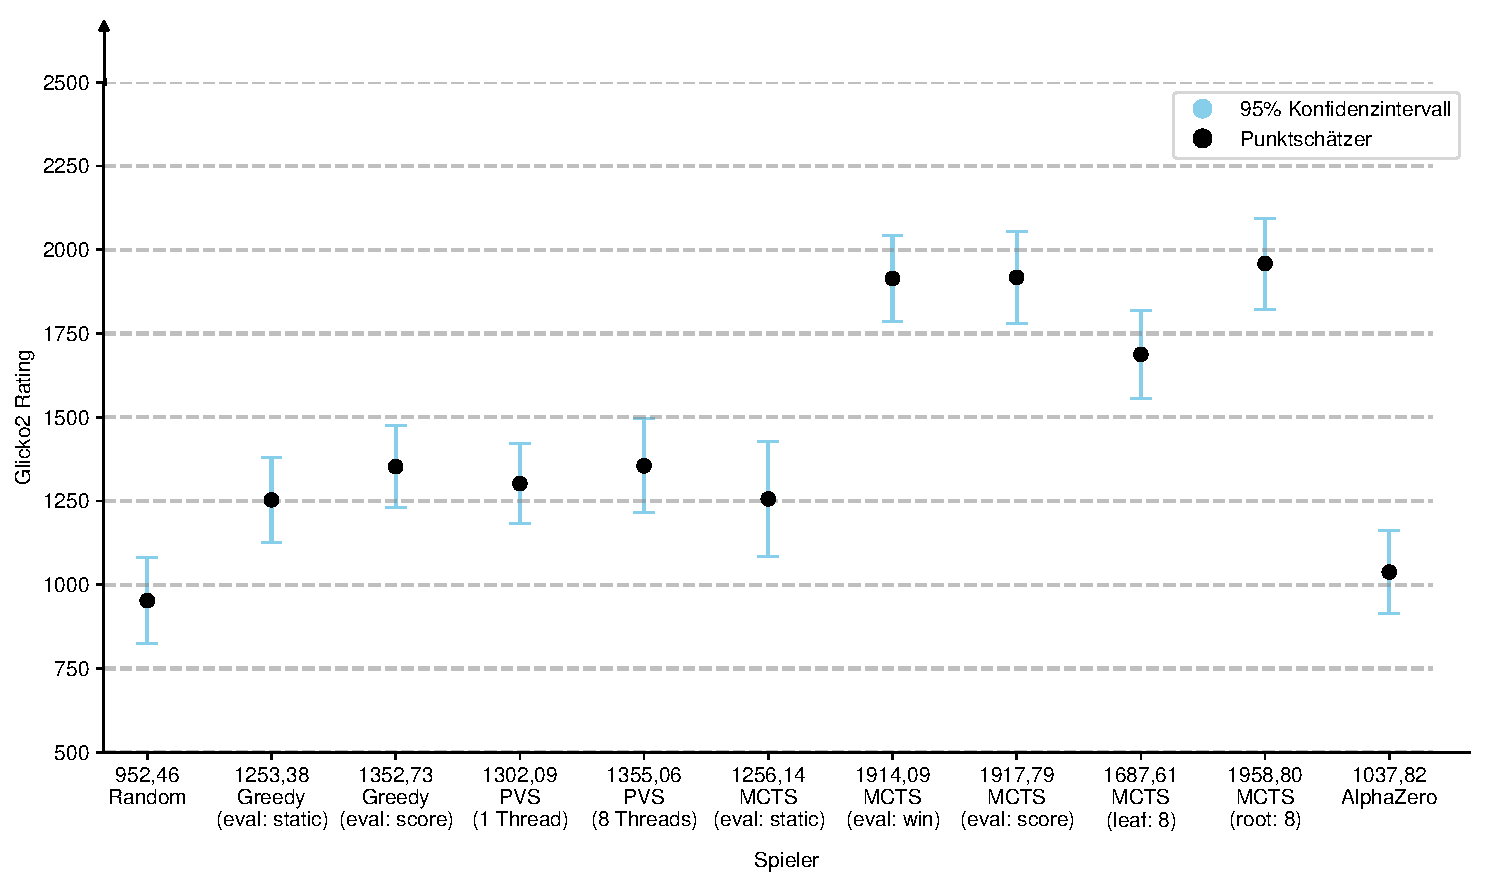
\includegraphics[width=\textwidth]{res/pictures/plots/player-ratings.pdf}
    \caption{Bewertung der Spieler im Glicko-2-Wertungssystem}
    \label{fig:player-ratings}
\end{figure}

TODO:

\section{Ergebnisse gegen die Autoren}

TODO: